\chapter{Problématique}\label{chap:intro}
\newpage
\minitoc
\newpage

\section{Présentation générale}\label{sec:pres}
Dans cet ebook (~ou livre électronique en bon français~), vous allez
découvrir ce qui est bien trop souvent passé sous silence dans les
cours de langues\ldots{} la \underline{phonétique} ! En effet, en France en
particulier\footnote{N'ayant jamais fait d'études à l'étranger je ne
  peux pas me permettre de parler des autres pays.}, les cours de
langues insistent rarement sur l'oral\footnote{Comme on peut le voir
  dans cet
  \href{http://doyouspeakenglish.fr/les-francais-savent-ils-parler-anglais/}{article}
  que j'ai écrit sur mon blog après avoir vu la vidéo que j'ai mis en
  début d'article accessible en cliquant sur ce lien 
  \url{http://doyouspeakenglish.fr/les-francais-savent-ils-parler-anglais/}.}. Attention, je parle des cours
de langue avant le bac. Il faut savoir que \underline{normalement}
l'objectif de l'enseignement obligatoire\footnote{En France
  l'instruction est obligatoire jusqu'à 16 ans ce qui correspond
  normalement à la classe de seconde ou troisième en cas de
  redoublement.} est d'atteindre le
\href{http://doyouspeakenglish.fr/quel-niveau-danglais-avez-vous/}{niveau
  B1} du cadre de référence européen\footnote{Bien entendu j'exclu les
classes dites <<~européennes~>> puisqu'elles ne représentent pas la
fillière standard mais plutôt l'exception qui confirme la règle.}. Hélas, la réalité est
loin d'être celle qu'espèrent les ministres et de nombreux indicateurs le prouvent :
\begin{itemize}
\item niveau en anglais par rapport aux autres pays
  \href{http://doyouspeakenglish.fr/les-francais-sont-ils-les-derniers-en-europe/}{européens}\footnote{Vous
    pouvez aller sur mon blog pour lire l'article consacré
    \url{http://doyouspeakenglish.fr/les-francais-sont-ils-les-derniers-en-europe/} .}(~derrière l'Espagne, la Grèce, la Bulgarie, la Roumanie\ldots{} voir la figure
  \ref{fig:1} page \pageref{fig:1} pour plus de détails~)
  \begin{figure}[h]
    \centering
    \caption[L'anglais en Europe]{Niveau d'anglais des
      pays européens}\vspace{.1cm}
    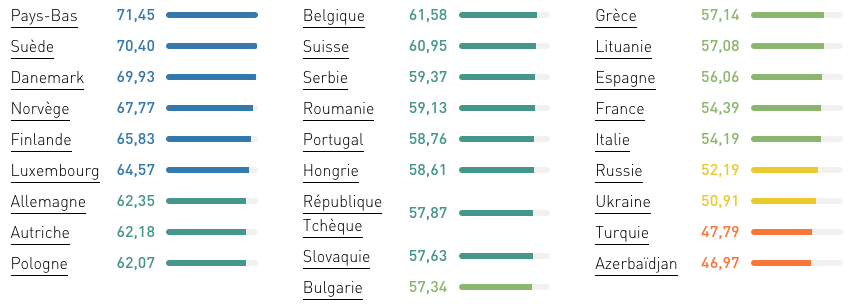
\includegraphics[scale=.5]{../img/french-english-level-in-europe}
    
    \label{fig:1}
  \end{figure}
\item niveau en anglais par rapport \href{http://doyouspeakenglish.fr/numero-1-en-tourisme-mais-dernier-en-anglais/}{au
    reste du monde}\footnote{Vous pouvez aller directement sur mon blog
  \url{http://doyouspeakenglish.fr/numero-1-en-tourisme-mais-dernier-en-anglais/} pour observer l'étude complète.}
(~derrière la République Dominicaine et la Corée du Sud s'il vous
plaît\ldots{} voir la figure \ref{fig:2} page \pageref{fig:2} pour
plus de détails~)
  \begin{figure}[h]
    \centering
    \caption[L'anglais dans le monde]{Niveau d'anglais dans le monde}\vspace{.1cm}
    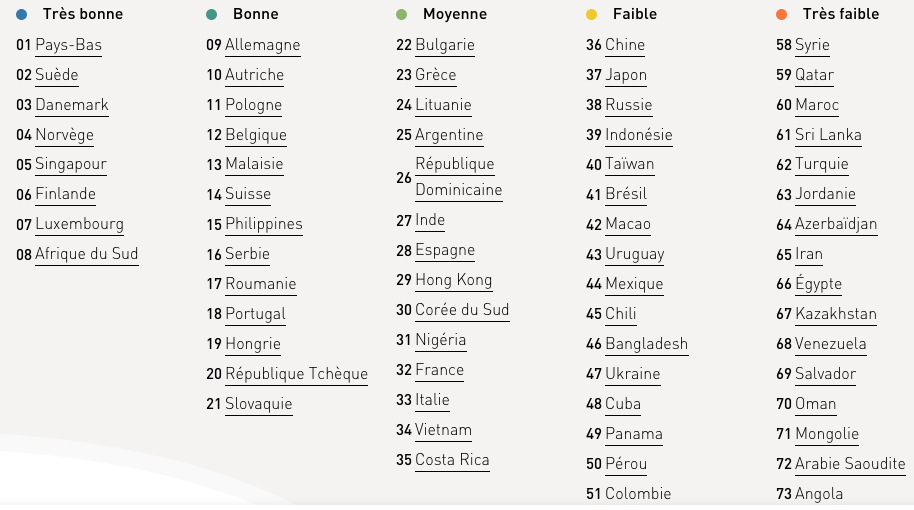
\includegraphics[scale=.5]{../img/english-level-in-the-world}
    
    \label{fig:2}
  \end{figure}
\item encore des
  \href{http://doyouspeakenglish.fr/les-francais-et-les-langues-en-quelques-chiffres/}{chiffres
    accablants}\footnote{Consulter mon article sur \url{http://doyouspeakenglish.fr/les-francais-et-les-langues-en-quelques-chiffres/}}
   
  \begin{figure}[h]
    \centering
    \caption[L'anglais en France]{Niveau d'anglais en France}\vspace{.1cm}
    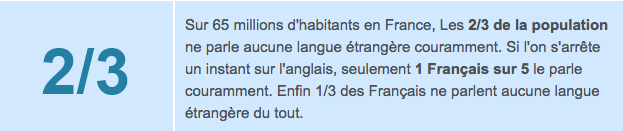
\includegraphics[scale=.725]{../img/french-english-level-in-france}
    
    \label{fig:3}
  \end{figure}
\end{itemize}
Loin de moi l'idée de vous assommer avec des chiffres et encore moins
de partir dans l'auto-flagellation. Néanmoins, il faut être lucide, il
y a un problème franco-français (~qui est très bien expliqué dans cet
\href{http://www.larevuedesressources.org/les-francais-et-les-langues-etrangeres,2920.html}{essai}~). 
Ce problème est très bien développé et analysé dans l'essai du
professeur Daniel Emilio Rojas\footnote{Lisez-le c'est gratuit, très
  bien écrit et instructif : \url{http://www.larevuedesressources.org/les-francais-et-les-langues-etrangeres,2920.html}} (~hispanophone natif qui parle et écrit
probablement beaucoup mieux le français que 90\% d'entre
nous~). Cependant, je me permettrais de vous proposer un raccourci\footnote{Forcément réducteur.} pédagogique en vous rappelant un fait
élémentaire mais que l'on oublie trop souvent. Parfois les solutions
sont tellement \underline{bêtes} qu'on oublie d'y penser. Attention, je ne
prétends pas vous proposer de recette miracle. L'anglais est une
langue difficile\footnote{Des linguistes professionnels et moi-même te
  le montrent dans cet article \url{http://doyouspeakenglish.fr/langlais-une-langue-facile/} }, bizarre, complexe et
illogique\footnote{Comme beaucoup de langues et notamment le
  français.}; et je ne suis pas le seul à le dire puisque certains anglophones natifs (~et
linguistes de surcroît~) le disent et l'écrivent par exemple dans cet \href{http://doyouspeakenglish.fr/langlais-une-langue-facile/}{article} qui permet également d'être
écouté\footnote{Comme je le montre dans cette vidéo
  \url{https://youtu.be/6wLbtx2iL7c}}. Donc oui l'anglais est
difficile, \underline{mais} avec un peu de bon sens et de persévérence
vous pouvez y arriver\footnote{Bon, il y a une triste vérité qu'il
  faut accepter, vous ne parlerez \underline{jamais} comme un natif (~\underline{sauf}
  si vous décidez de vous installer dans un pays anglophone~).}. 

\newpage
\section{Le truc tout bête}\label{sec:truc}
Mais quel est donc ce truc \underline{tout bête} que l'on oublierait et dont je
ne vous ai toujours pas parlé ? Minute papillon ! Non ! Je n'essaie
pas de noyer le poisson, je vais vous révéler mon \underline{truc}. Je vous
préviens, vous allez être probablement déçu, mais pourtant c'est une
évidence. \par
Allons-y ! Et bien, je ne sais pas pour vous mais pour moi\footnote{Et il me
semble pour la plupart des gens aussi.}, l'acquisition de ma langue
maternelle a commencé par l'oral et non par l'écrit. Pendant au moins
5 ans\footnote{Avant l'entrée au CP ou tout autre système scolaire qui
apprend à lire et à écrire.}, j'ai pratiqué en priorité l'écoute et la
méthode essai/erreur\footnote{En anglais on dit \exEN{try and guess} ce qui veut
dire \exFR{essayer et deviner}, qui est un point de vue plus positif (
attitude plus répandue chez les anglophones et en particulier chez les américains).}. Ben
oui, quand on est enfant on baigne dans un environnement linguistique
oral. Et dès les premiers mois de la vie on essaie (~avec beaucoup de
difficultés au début~) de produire ou plutôt reproduire des \textcolor{teal}{sons} que
l'on a entendu. Et croyez-moi, si vous avez oublié allez faire un tour
chez votre frère, soeur, cousin, cousine, ami, amie qui a (~ont~) des
enfants en bas âge et cela vous raffraichira la mémoire. La parole est
si importante pour l'humanité qu'elle a été pendant des siècles (~ des
millénaires même!~) le seul et unique vecteur de
communication. D'ailleurs aujourd'hui encore parmi les presque 7~000
\href{http://www.museedelhomme.fr/fr/combien-langues-sont-parlees-monde}{langues dans le monde} la plupart ne possèdent pas de système
d'écriture. Pour plus de précisions sur la répartition linguistique
dans le monde vous pouvez consulter \href{http://www.axl.cefan.ulaval.ca/Langues/1div\_recens.htm}{ce site canadien} qui tire ses
sources statistiques du \underline{Summer Institute of Linguistics} du
Texas\footnote{Voici l'url du site
  \url{http://www.axl.cefan.ulaval.ca/Langues/1div_recens.htm}}
(~2017~). Et avec l'avènement de la reconnaissance vocale il se
pourrait bien que l'écriture devienne un art au même titre que la
calligraphie et non plus une compétence indispensable.

\newpage

\subsection{Quelques citations}\label{subsec:quote}

% \begin{bigquote}[1.0]
%   \begin{displayquote}[Extrait du livre \FL.][.]
%     Les Romains, déjà, ne parlaient pas exactement la langue qu'ils
%   écrivaient. Ainsi, \underline{cheval} vient d'un mot parlé,
%   \exLT{caballus}, alors que le latin classique écrit \exLT{equus} ---
%   d'où viendront des mots <<~savants~>> comme \underline{équidé} et
%   \underline{équitation}
%   \end{displayquote}
% \end{bigquote}  

\begin{mdframed}[style=citestyle, frametitle={Extrait du livre \FL.}]
  Les Romains, déjà, ne parlaient pas exactement la langue qu'ils
  écrivaient. Ainsi, \underline{cheval} vient d'un mot parlé,
  \exLT{caballus}, alors que le latin classique écrit \exLT{equus} ---
  d'où viendront des mots <<~savants~>> comme \underline{équidé} et
  \underline{équitation}.
\end{mdframed}

D'ailleurs comme le montre la première vidéo dans
\href{http://doyouspeakenglish.fr/prescriptiviste-ou-descriptiviste/}{cet
  article}, les zones du cerveau actives pour la parole et pour l'écriture sont différentes.\par

\begin{mdframed}[style=citestyle, frametitle={Extrait du livre \FL.}]
  Longtemps, le français s'est écrit comme il se parlait; vice versa,
  toutes les lettres se prononçaient, comme en latin. La notion même
  d'orthographe n'existait pas.
\end{mdframed}

En lisant ce dernier extrait je parie que certains d'entre vous sont en train
de chercher un moyen pour inventer une machine à remonter le temps. 

Vous vous demandez sûrement où je veux en venir. Mon but est de vous
faire comprendre ou plutôt de vous rappeler qu'une langue ça s'écoute
et ça se parle pendant un certain temps (~jusqu'à ce que ça devienne
naturel~) avant d'apprendre à l'écrire et d'étudier toutes les
subtilités de la grammaire. \href{https://fr.wikipedia.org/wiki/Django\_Reinhardt}{Django Reinhardt} et \href{https://fr.wikipedia.org/wiki/Louis\_Armstrong}{Louis Amstrong} ne
savaient ni lire ni écrire la musique et pourtant ils sont des
musiciens vénérés de leur vivant et encore aujourd'hui.\par

\newpage

\section{Une langue est une musique}\label{sec:music}
Et oui une langue c'est également une musique ! Une langue a une
musicalité et un rythme. Pas de chance pour nous le français (~ou
plutôt le \underline{parisien}\footnote{J'en parlerais plus en détails
  dans un prochain livre mais si vous êtes impatient alors je vous
  recommande de vous procurer \FL.}~)
n'est pas très chantant. Mais pourtant si l'on écoute les accents du
midi il y a tout de suite plus de mélodies qui chatouillent nos
oreilles. 

En résumé, ce que je vais partager avec vous dans ce livre, ce
sont les \textcolor{teal}{sons} de la langue anglaise. Les \href{https://pronunciationstudio.com/45-Sounds/}{45 \textcolor{teal}{sons}} (~certains en
décrivent 44, pour le français\footnote{Selon le \GE il y a 36 \textcolor{teal}{sons}
  <<~\exFR{purement}~>> français auquel on ajoute le \son~\phon{ŋ}
  hérité de l'anglais et notamment utilisé dans \exEN{parking}.} c'est
pareil, certains disent 36 d'autres 37~) de la langue anglaise telle
qu'elle est parlée en Angleterre et je préciserai également les
distinctions qu'il convient de noter par rapport à l'anglais
américain. En tant que français nous sommes beaucoup plus proche de
l'Angleterre (et des Îles Britanniques en général) que des
\'Etats-Unis.

Néanmoins, il est certain qu'avec les productions américaines au
cinéma, à la télévision, ou sur Internet nous sommes plus souvent
confrontés à de l'anglais américain. Mais par contre tous les examens
comme le TOEFL ou le TOEIC portent sur l'anglais britannique. 

%\begin{itemize}
% \item Dans une première partie je vous présenterai la phonétique du
% français. En effet, il me semble plus judicieux d'approcher ce nouvel
% ensemble de symbole qui décrit les \textcolor{teal}{sons} avec précisément des \textcolor{teal}{sons} que
% vous utilisez déjà tous les jours.
Pour conclure cette introduction je rappelerai deux faits que l'on a tendance à oublier mais qu'il faut \underline{absolument garder à l'esprit} :

\begin{enumerate}
\item Le français est une langue syllabique alors que l'anglais est
  une langue accentuelle\footnote{Consulter mon \href{http://doyouspeakenglish.fr/laccent-tonique-en-anglais/}{article} de
    blog pour plus de détals.}.
\item En français il y a 36 \textcolor{teal}{sons}\footnote{Selon le
    \GE 36 mais selon Sousa auteur du livre \HTEBL il
    n'y en aurait que 32. Pour ce chiffre j'accorderai plus de crédit
    au \GE pour la bonne et simple raison qu'en tant que linguiste
    francophone il me semble plus compétant que Sousa qui est
    anglophone.} et 250 façons\footnote{Encore une fois les
    estimations diffèrent \GE n'en compte que 130 ce qui accentue
    encore plus la complexité de l'anglais.} de les écrire alors qu'en
  anglais il y a 44 \textcolor{teal}{sons} pour 1~100 façons de les écrire\footnote{Les
    chiffres concernant les façons d'écrire sont issus des
    comparaisons présentées dans le livre \HTEBL Chapter 4 Teaching
    English Language Reading and Writing page 84 Table 4.1.}.
\end{enumerate}

Par conséquent \underline{la prononciation, l'accent et le rythme} ne sont pas
superflus mais \underline{obligatoire en anglais}.\par

% Dans la deuxième partie du livre je vais vous présenter 45
% \textcolor{teal}{sons} qui sont absolument \underline{fondamentaux}
% dans la langue anglaise. En insistant particulièrement sur ceux qui
% n'apparaissent pas du tout dans la langue française.
% Et pour bien
% faire la différence il était important de commencer par la phonétique
% de la langue française que vous ne connaissez probablement pas
% encore. C'est pour cette raison qu'il est vivement recommandé de lire ce livre dans l'ordre.
%\end{itemize}

\newpage
\section{Mini conclusion de cette introduction}\label{sec:mini}
J'ai dit qu'on apprend d'abord à parler avant d'écrire, c'est vrai,
mais a priori, si vous lisez ce livre c'est que vous savez lire. Et
comme vous savez lire et bien on va en profiter pour apprendre encore
plus efficacement en utilisant
l'\href{https://fr.wikipedia.org/wiki/Alphabet_phon\%C3\%A9tique_international}{API}\CW{https://fr.wikipedia.org/wiki/Alphabet_phon\%C3\%A9tique_international}
(~Alphabet Phonétique International~). En anglais on l'écrit
IPA\CW{https://en.wikipedia.org/wiki/International_Phonetic_Alphabet}
(~International Phonetic Alphabet~).\par

Et cerise sur le gâteau, ceci vous sera utile pour toutes les autres
langues que vous souhaitez apprendre ou que vous parlez déjà (~cela va
même améliorer votre français~).

D'ailleurs, contrairement à ce que certaines personnes pourraient
penser, apprendre une autre langue, et en particulier l'anglais,
améliore votre niveau de français\footnote{En effet il existe plus de
  25~000 mots anglais d'origine française et vous pouvez en découvrir
  quelques-uns grâce aux cartes mémoires que j'ai créé :   \url{https://tinycards.duolingo.com/decks/6VNKUdba/english-words-with-french-origin}
  et au livre plus complet \HSQMYP.}.

En effet, lorsqu'on apprend une langue étrangère on commence toujours
par la comparer avec notre langue maternelle ce qui implique
l'observer à travers ses règles. Par conséquent on redécouvre les
structures propres à notre langue maternelle ce qui renforce nos
connaissances sur le sujet. Ce n'est pas magique, mais c'est
véridique. Alors c'est parti, allons découvrir les 45
\textcolor{teal}{sons}\footnote{Vous pouvez déjà vous entraîner
  grauitement grâce aux cartes mémoires que j'ai créé : \url{https://tiny.cards/decks/6YTEvyrN/english-phonetics}}
de la langue anglaise (~qui n'a plus grand chose à voir avec 
Shakespeare de la même manière qu'on ne parle plus la langue de
Molière~). Mais avant ça je vais vous présenter quelques notions un peu
abstraites mais utiles. 

\newpage
\minitoc
